\documentclass[xcolor=table, compress, %
handout
]{beamer}

\usetheme{Luebeck}
\usepackage{beamerthemesplit}
\usecolortheme{beaver}
\setbeamercolor{navigation symbols}{fg=black, fg=gray}
\setbeamercolor{structure}{fg=gray}
\setbeamercolor{alerted text}{fg=darkred}
\resetcounteronoverlays{exx}

\usepackage{setspace}
\usepackage{relsize}
\usepackage{pgfpages}
\usepackage{graphicx}
\usepackage{booktabs}
\usepackage{subfigure}	% mehrere Bilder in einer figure-Umgebung
\usepackage{marvosym} %Radioaktiv-Zeichen
\usepackage[english, ngerman]{babel}
%\usepackage{beamerthemesplit}

%\usepackage{lmodern,textcomp}

\usepackage{fontspec}
\setromanfont{CMU Serif}
\setsansfont{CMU Sans Serif}
\setmonofont{CMU Typewriter Text}

\usepackage{tikz}
\usepackage{tikz-qtree}
\usepackage{tikzducks}

\usepackage{tipa}
\usepackage{verbatimbox} % Muss bei beamer als \begin{frame}[fragile] gekennzeichnet werden


%% biblatex-Optionen und Gestaltung der Bibliographie
\usepackage[style=authoryear-comp, natbib=true, maxcitenames=3, backend=biber]{biblatex}
\bibhang1em
%\usepackage[babel, english=quotes]{csquotes}
\DeclareFieldFormat{postnote}{#1}%--> kein S. in Zitaten
\DeclareFieldFormat{multipostnote}{#1}%--> kein S. in Zitaten
\renewcommand*{\postnotedelim}{\addcolon\addspace}%%--> : statt , in Zitaten
\DeclareFieldFormat{pages}{#1} %%--> kein S. in Bibliographie
\renewcommand*{\bibpagespunct}{\addcolon\addspace} %%--> : in Bibliographie statt ,
\bibliography{BibliographieNegation.bib}

\usepackage[babel, german=quotes]{csquotes}
\usepackage{ragged2e}

%Linguistik-Pakete%
\usepackage{expex}
\usepackage{gb4e}
\usepackage{xcolor}

%neue Kommandos Oliver%
\newcommand{\qu}[1]{„#1“}
\newcommand{\qufs}[1]{,#1‘}
\newcommand{\tsub}[1]{\textsubscript{#1}}
\newcommand{\tsup}[1]{\textsuperscript{#1}}
\newcommand{\tuple}[1]{$\langle$#1$\rangle$}
\newcommand{\blau}[1]{{\color{blue} #1}}
\newcommand{\rot}[1]{{\color{red} #1}}
\def\newblock{\hskip .11em plus.33em minus.07em}
\let\eachwordone=\sf  % Schriftart bei Glossen bleibt bei Übergängen gleich
\let\eachwordtwo=\sf  %
\newcommand{\oldoe}{$\stackrel{\textsf{\tiny e}}{\textsf{o}}$}

\setbeamercolor{alerted text}{fg=orange}

\newcommand*{\ballref}[1]{%
    \begin{pgfpicture}{-1ex}{-0.65ex}{1ex}{1ex}
    \usebeamercolor[fg]{item projected}
    {\pgftransformscale{1.75}\pgftext{\normalsize\pgfuseshading{bigsphere}}}
    {\pgftransformshift{\pgfpoint{0pt}{0.5pt}}
      \pgftext{\usebeamerfont*{item projected}\ref{#1}}}
  \end{pgfpicture}}%
  
  % Edh und Thorn
\DeclareTextSymbolDefault{\dh}{T1}
\DeclareTextSymbolDefault{\th}{T1}


\title[Loss of the MHG bipartite negation marker \textit{ne ... niht}]{\bf{The loss of the MHG bipartite negation marker \textit{ne ... niht}}}
\subtitle{Diachronic and diatopic variation in ReM and CAO}
\author[Daniel Hrbek and Oliver Schallert]{%
Daniel Hrbek\inst{1} \and Oliver Schallert\inst{2}}
\institute{%
\inst{1} Osnabrück University %\\ Institut für Germanistik \\ 

\href{mailto:daniel.hrbek@uni-osnabrueck.de}{\texttt{daniel.hrbek@uni-osnabrueck.de}}
\and
\inst{2} Ludwig Maximilian University of Munich %\\ Institut für Deutsche Philologie \\ 

\href{mailto:oliver.schallert@lmu.de}{\texttt{oliver.schallert@lmu.de}}
}

\date{02.\,07.\,2022
}
\pgfdeclareimage[width=2.5cm]{logo}{LMU-Logo.png}
% Logo Uni Osnabrück ergänzen
 \pgfdeclareimage[width=3.75cm]{pogo}{UOS-R.jpg} 
% \pgfdeclareimage[width=3.75cm]{pogo}{UOS-SW.jpg} 
% \pgfdeclareimage[width=3.75cm]{pogo}{UOS-SWR.png} 
\titlegraphic{\vspace{-0.2cm}\pgfuseimage{pogo}\hspace{0.5cm}\pgfuseimage{logo}}

\begin{document}

\begin{frame}
\titlepage
\end{frame}



\begin{frame}{Roadmap}

\tableofcontents[sections={1-2}]

\end{frame}

\begin{frame}{Roadmap}

\tableofcontents[sections={3-5}]


\end{frame}

\begin{frame}{Acknowledgement}

For numerous tips and helpful conversations as well as the preview of her PhD thesis:

\begin{itemize}
\item \alert{Julia Hertel} (née Schüler) (Saarland University) for a preview of her PhD thesis
\end{itemize}
\bigskip

Collaboration Document Project:
\begin{itemize}
\item \alert{Carsten Becker,} University of Marburg
\end{itemize}

\end{frame}


\section{Point of departure}

\begin{frame}{Point of departure}

\pex[interpartskip=1ex] \label{a}
\a
\begingl
\gla die \textbf{ne}mugin iz uernemen//
\glb they NEG=could it hear//
\glft Wiener Physiologus (149va,5)//
\endgl
\a
\begingl
\gla er\textbf{ne} wil dich \textbf{nit} lazen//
\glb he=NEG wants you NEG let//
\glft Rolandslied (0a,8969)//
\endgl
\a
\begingl
\gla Sí	ſprachen \textbf{niht} an dem hilígen tag//
\glb they talked NEG on the sacred day//
\glft  Oberaltaicher Evangelistar (25ba,37)//
\endgl
\xe

\end{frame}

\begin{frame}{Point of departure}
\framesubtitle{Negation structures in the course of German}

In all Old Germanic languages, we find a preverbal negation particle \textit{ni}/\textit{ne} that derives from PTG \textit{*ni} (cf. \citealt{Eythorsson1995}, \citealt{Eythorsson2002}):

\pex
\a
\begingl
\gla ni was wul\th ag//
\glb \textsc{NEG} was glorious//
\glft Gothic; 2nd Letter Corinthians 3:10//
\endgl
\a
\begingl
\gla ni láz thir nan ingángan//
\glb \textsc{NEG} let you him escape//
\glft OHG; Otfrid IV 37,11//
\endgl
\a
\begingl
\gla út \th ú ne komir / órum h\textipa{\k{o}}llum frá//
\glb out you \textsc{NEG} come {} our.\textsc{DAT.PL} hall.\textsc{DAT.PL} from//
\glft Old Norse; Vaf\th rú\dh nismál 7//
\endgl
\xe

\end{frame}

\begin{frame}{Point of departure}
\framesubtitle{Negation structures in the course of German}

\citet[690]{Grimm1890} already noted that the early Germanic dialects are strikingly similar in matters of negation:
\bigskip
\par
\begingroup
\leftskip=0.5cm % Parameter anpassen
\noindent %ab hier der Text, der eingerückt werden soll
\begingroup
\rightskip=0.5cm % Parameter anpassen
\noindent %ab hier der Text, der eingerückt werden soll

\begin{small}
NI war die ursprüngliche und wahre negation; in der goth sprache hat sie noch den weitesten spielraum, in den übrigen nimmt sie allmählich ab, wiewohl auf verschiedne weise; heutzutag ist sie vor dem verbo überall verschwunden und den partikeln gewichen, die anfangs bloss zu ihrer verstärkung hinter das verbum gestellt wurden und zum theil mit ihr selbst zusammengesetzt sind. 
\end{small}

\par
\endgroup
\par
\endgroup 

\end{frame}

\section{Diachrony of \textit{Jespersen's Cycle} in German}
\subsection{\textit{Jespersen's Cycle} in general}

\begin{frame}{Diachrony of \textit{Jespersen's Cycle} in German}
\framesubtitle{\textit{Jespersen's Cycle}}

\begin{figure}[h]
\centering
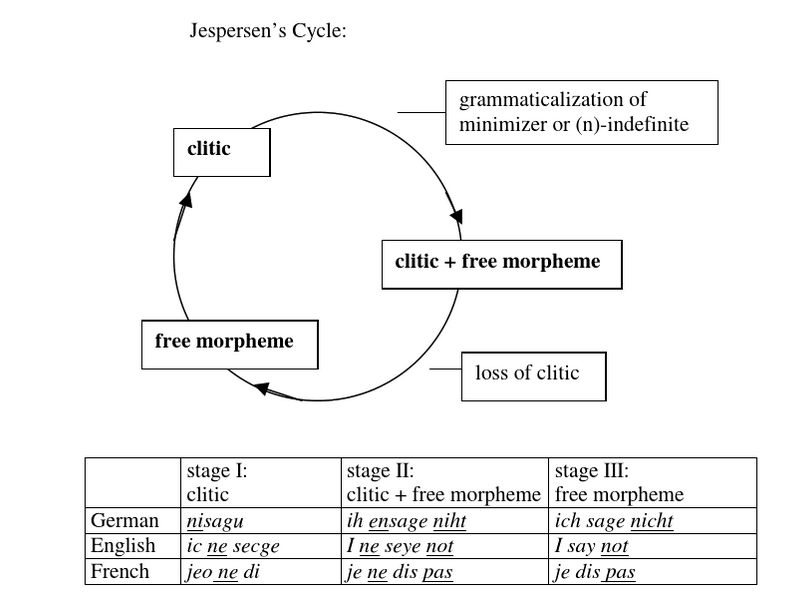
\includegraphics[width=8.5cm]{Jespersen.png}
\caption{\textit{Jespersen's Cycle} (\citet[15]{jaeger08})}
\end{figure}
\begin{itemize}
    \item The \textit{Jespersen's Cycle} (\citealt{jespersen17}) can be observed in all of the Germanic languages: ptg. *\textit{ni} (< ie. *\textit{ne}) $>$ me. \textit{ne ... nought}, on. \textit{ne ... -at/eigi} $>$ engl. \textit{not}, isl. \textit{ekki}
\end{itemize}

\end{frame}

\begin{frame}{Diachrony of \textit{Jespersen's Cycle} in German}
\framesubtitle{\textit{Jespersen's Cycle}}
\textit{Jespersen's Cycle} consists of \textbf{three stages} which can be observed in \textbf{every West Germanic language}:

\begin{itemize}
    \item \textbf{Stage I:} the single preverbal element OHG \textit{ni} gets (phonologically) weakened $\rightarrow$ MHG \textit{ne/en}
    \item \textbf{Stage II:} now weakened \textit{ne} is found insufficient to express negation on its own and is therefore strengthened by an additional element MHG \textit{niht} ($<$ OHG \textit{niouuiht} ‚nothing‘) $\rightarrow$ \textbf{bipartite negation marker} \textit{ne ... niht}
    \item \textbf{Stage III:} the original element falls victim to complete loss $\rightarrow$ MHG \textit{niht} expresses (sentential) negation on its own
\end{itemize}

\end{frame}

\subsection{Previous studies}
\begin{frame}{Diachrony of \textit{Jespersen's Cycle} in German}
\framesubtitle{Previous studies}

\begin{itemize}
    \item For a long time, \textit{Jespersen's Cycle} was accepted for entire West Germanic.
    \item This was recently proven for e.g. Low German by \citet{Breitbarth2014}.
    \item Therefore, MHG was assumed to be a Stage II language: \textit{ne ... niht} as the main strategy of negation.
    \item However, recent studies for MHG (\citealt{jaeger08,Pickl2017}) reveal that MHG scenario is significantly more complex.
\end{itemize}

\end{frame}

\begin{frame}{Diachrony of \textit{Jespersen's Cycle} in German}
\framesubtitle{Previous studies}

\begin{itemize}
    \item Jägers (\citeyear{jaeger08}) data suggest that MHG finished \textit{Jespersen's Cycle} at the end of the 13th century – at the latest!
    \item Pickls (\citeyear{Pickl2017}) prayers study support Jägers findings for Upper German $\rightarrow$ \textit{niht} as the main negation strategy already by 1200!
    \item However, \citet{witzenhausen19} (\textit{ne} only) and \citet{schueler16}/\citet{HertelimErscheinen}, who analyzed MHG charters (incl. Western Central German dialects) both state a high amount of areal variation!
\end{itemize}

\end{frame}

\begin{frame}{Diachrony of \textit{Jespersen's Cycle} in German}
\framesubtitle{Previous studies}

\begin{center}
\begin{tabular}{c c c c}
\hline\hline
 & \textbf{Bipartite negation} & \textbf{single \textit{niht}} & \textbf{total}\\
\hline
Cologne & 64 (94,1\%) & 4 (5,9\%) & 68 (100\%)\\
Regensburg & 6 (5,5\%) & 103 (94,5\%) & 109 (100\%)\\
Zürich & 1 (1,3\%) & 78 (98,7\%) & 79 (100\%)\\
\hline
total & 71 (27,6\%) & 186 (72,4\%) & 256 (100\%)\\
\hline\hline
\end{tabular}
\end{center}
\begin{small}
\begin{center}\smallskip
Table: Variation in sentential negation in MHG charters by 1280 (\citealt[98]{schueler16})\end{center}
\end{small}
\end{frame}

\subsection{Open issues}
\begin{frame}{Diachrony of \textit{Jespersen's Cycle} in German}
\framesubtitle{Open issues}

Previous research paints an unclear picture:

\begin{itemize}
    \item So far, we know that \textit{Jespersen's Cycle} underlies a strong areal variation in MHG.
    \item While UG becomes a stage III language by 1250, CG remains a stage II language by the end of MHG.
    \item Triggers for \textit{Jespersen's Cycle} are still unclear; previous studies suggest syntactic (\citealt{jaeger08,Breitbarth2014}) as well as phonological (\citealt{HertelimErscheinen}) factors.
    \item Both accelerating and retarding factors need further investigation.
\end{itemize}

\end{frame}

\begin{frame}{Diachrony of \textit{Jespersen's Cycle} in German}
\framesubtitle{Open issues}

\begin{itemize}
    \item Therefore, we will present results from our two corpus-based studies:
    \item \textbf{Referenzkorpus Mittelhochdeutsch} (ReM; ‚Reference Corpus of MHG‘) (1050–1350)
    \item \textbf{Corpus der altdeutschen Originalurkunden bis zum Jahre 1300} (CAO; ‚Corpus of Old German Original Charters until the year 1300‘)
\end{itemize}

\end{frame}

\section{Our database}
\subsection{Reference Corpus of MHG}
\begin{frame}{Our database}
\framesubtitle{Reference Corpus of MHG}

    \begin{itemize}
        \item \textbf{\textit{Referenzkorpus Mittelhochdeutsch}} (ReM; \citealt{kleinetal16,Klein2016}): freely available since 2016, contains texts (written between 1050 and 1350) from the entire Middle High German area 
        \item contains about two million tokens and is PoS-tagged
        \item consists of \textbf{well-balanced text genres} (e.g. Chivalric romance, prayers, charters or recipes) $\rightarrow$ text type-specific influences can be kept low
         \item However, in \textbf{diachronic and diatopic matters}, the ReM is \textbf{not well-balanced}: Western Central and Eastern Upper German predominate and early texts are scarce.
          \begin{itemize}
              \item[\Radioactivity] Analyzing Eastern Central German is particularly problematic since these dialects were formed only a few centuries ago.
              \item[\Radioactivity] Therefore, we will exclude ECG for the most part!
          \end{itemize}
    \end{itemize}

\end{frame}

\begin{frame}{Our database}
\framesubtitle{Reference Corpus of MHG}

    \begin{itemize}
        \item Although it uses ANNIS3 (\citealt{Krause2016}), ReM  \textbf{lacks syntactic annotations}. $\rightarrow$ limited use for complex syntactic phenomena
        \item Furthermore: Crashes/overloads and occasional errors/bugs $\rightarrow$ ReM \textbf{doesn't run smoothly in some places yet}
        \item Many queries for syntactic phemona must be substituted (e.g. with distance parameters)
        \item For the syntactic variation: sample of 501 instances of \textit{ne ... niht} (using \textit{R}'s \textit{dplyr})
        \item Results presented here taken from \citet{hrbek21}
    \end{itemize}

\end{frame}

\subsection{Corpus of Old German Original Charters}
\begin{frame}{Our database}
\framesubtitle{Corpus of Old German Original Charters}

\begin{itemize}
   \item \textbf{Corpus der altdeutschen Originalurkunden bis zum Jahre 1300} (CAO; Wilhelm et al. \citeyear{cao1}–\citeyear{cao5})
    \item allows observation of diatopic differences from  1250 to 1300
    \item \citet{beckerschallert21,beckerschallert22a,beckerschallert22b}, \citet{HertelimErscheinen}
\end{itemize}

\end{frame}

\section{Involved factores in discussion}
\begin{frame}{Involved factores in discussion}

Before we take a closer look into our findings, we have to discuss a few phenomena which influenced the deletion of MHG \textit{ne} and \textit{ne ... niht}:

\begin{itemize}
    \item \textbf{Phonological aspects} which caused \textit{ne} to disappear and
    \item \textbf{Morphosyntactic aspects} which accelerated or delayed this development.
\end{itemize}

\end{frame}

\subsection{Phonological aspects}

\begin{frame}{Involved factores in discussion}
\framesubtitle{Phonological aspects}

During MHG, there are mainly two phonological developments which contradict a long lasting bipartite negation marker:

\begin{itemize}
    \item \textbf{Reduction of unstressed syllables}: Since late OHG, unstressed syllables with full vowels (such as /a/, /i/, /u/) are slowly reduced to Schwa (/\textipa{@}/).
    \begin{itemize}
        \item This development continued until the end of MHG and was subject to a large areal variation.
        \item While UG was covered quickly and comprehensively, the reduction in CG was significantly delayed.
    \end{itemize}
\end{itemize}

\pex
\a
OHG \textit{sunna} $\rightarrow$ MHG \textit{sunne}
\a
OHG \textit{umbigeban} $\rightarrow$ MHG \textit{umbegeben}
\xe

\end{frame}

\begin{frame}{Involved factores in discussion}
\framesubtitle{Phonological aspects}

\begin{itemize}
    \item \textbf{Schwa (/\textipa{@}/) deletion}: During MHG, Schwa was deleted in reduction syllables and (prosodically) weak functional words (such as particles).
    \begin{itemize}
        \item \textit{ne} as a functional word was hit systematically: \textit{ne} $\rightarrow$ \textit{n} $\rightarrow$ \textit{en}
        \item single /n/ could not survive; a so-called \glqq Stützvokal\grqq{} (\citealt{Nuebling1992}, Paul et al. \citeyear{paul07}) had to be inserted $\rightarrow$ reduction to /\textipa{@}/ and deletion all over again
        \item From this perspective, MHG \textit{ne} was doomed to death.
    \end{itemize}
\end{itemize}

\pex
\a
early MHG \textit{kel.be.re} $\rightarrow$ late MHG \textit{kel.ber}
\a
OHG \textit{ni} $\rightarrow$ early MHG \textit{ne} $\rightarrow$ \textit{n} $\rightarrow$ late MHG \textit{en}
\xe

\end{frame}

\begin{frame}{Involved factores in discussion}
\framesubtitle{Phonological aspects}

\begin{itemize}
    \item Both developments can be found in the entire MHG area; however, it first started in UG and then slowly spread to CG (\citealt{Triwunatz1913}, \citealt{lindgren53}, \citealt{Klein2005}, \citealt{Buethe-Scheider2017}).
    \item Completed \textbf{during the 13\textsuperscript{th} century in UG}, but \textbf{not until early 16\textsuperscript{th} century for CG}. 
    \item[\Radioactivity] Until the development is completely finished, MHG \textit{ne} (as well as \textit{ne ... niht}) remained a \textit{dead man walking}.
\end{itemize}

\end{frame}

\begin{frame}{Involved factores in discussion}
\framesubtitle{Phonological aspects}

\begin{itemize}
    \item One more phonological development – \textbf{fixed metric trochee:} 
    \item During MHG, the trochee (\textipa{\'xx}) becomes more and more fixed $\rightarrow$ targeted intonation structure
    \item In order to maintain a trochee in (morphologically) complex words, syllables get deleted:
\end{itemize}

\pex
\a
wehsele   $>$  wechsel\alert{\emptyset} ‘exchange’\\
(($\sigma$\textsubscript{s}$\sigma$\textsubscript{r}\alert{$\sigma$\textsubscript{r}})\textsubscript{F})\textsubscript{$\omega$} $>$   (($\sigma$\textsubscript{s}$\sigma$\textsubscript{r}\alert{\emptyset})\textsubscript{F})\textsubscript{$\omega$}
\a
b. manete $>$ man\alert{\emptyset}te ‘admonished.{\textsc{3SG}}’\\
(($\sigma$\textsubscript{s}\alert{$\sigma$\textsubscript{r}}$\sigma$\textsubscript{r})\textsubscript{F})\textsubscript{$\omega$} $>$   (($\sigma$\textsubscript{s}\alert{\emptyset}$\sigma$\textsubscript{r})\textsubscript{F})\textsubscript{$\omega$}
\xe

\end{frame}

\begin{frame}{Involved factores in discussion}
\framesubtitle{Phonological aspects}

\begin{itemize}
    \item (Morphologically) simple words (e.g. Sg. Nom.) containing two (or more) syllables lose one (already reduced) syllable
    \item This is in order to form a trochee in more complex scenarios (e.g. Pl. Gen.).
    \item This holds true for functional words such as conjuncts and particles.
\end{itemize}
\vspace{-0.5cm}
\begin{figure} 
\begin{minipage}[t]{0.4755\textwidth}
\pex a. swane    $>$ swan ‘swan’\\
(($\sigma$\textsubscript{s}$\sigma$\textsubscript{r})\textsubscript{F})\textsubscript{$\omega$}  $>$ 
        (($\sigma$\textsubscript{s}\alert{\emptyset})\textsubscript{$\omega$}
\end{minipage}
\begin{minipage}[t]{0.475\textwidth}
\exdisplay b. vnde         $>$ vnd ‘and’\\
(($\sigma$\textsubscript{s}$\sigma$\textsubscript{r})\textsubscript{F})\textsubscript{$\omega$}  $>$ 
         (($\sigma$\textsubscript{s}\alert{\emptyset})\textsubscript{$\omega$}
\end{minipage} 
\end{figure}

\end{frame}

\subsection{Morphosyntactic aspects}
\begin{frame}{Involved factores in discussion}
\framesubtitle{Morphosyntactic aspects}
Previous studies (\citealt{behaghel18,Gaertner1977,Pickl2017}; \citealt{schueler16,schueler17}, \citealt{hrbek21}) discuss the following points:

\begin{itemize}
    \item bipartite negation marker \textit{ne ... niht} mainly attested in Western Central German texts ...
    \item ... and early loss / no use in Upper German texts
    \item early loss in V1 clauses, preservation in VF clauses
    \item (morphologically) complex verbs with prefixes (such as participles) tend to accelerate the loss of \textit{ne}/\textit{en}
\end{itemize}

\end{frame}

\begin{frame}{Involved factores in discussion}
\framesubtitle{Morphosyntactic aspects}

All of these aspects can be explained with Hertels \citeyear{HertelimErscheinen} prosody based approach:

\begin{itemize}
    \item \textit{ne} as a weak functional word gets reduced and fells victim to /\textipa{@}/-deletion quickly.
    \item In V1 clauses with \textit{ne}, the first syllable is unstressed – no trochee possible!
    \item The same holds true for prefixed verbs (espc. with an reduction syllable like \textit{ge-})!
    \item VF clauses, on the other hand, preserve the MHG trochee $\rightarrow$ last resort for \textit{ne ... niht}
\end{itemize}

\end{frame}

\section{Our results}

\subsection{Diachronic variation (ReM)}
\begin{frame}
\frametitle{Our results}
\framesubtitle{Diachronic variation (ReM)}
    
    \begin{itemize}
        \item \textit{Jespersen's Cycle} (all three stages) can be observed in many West Germanic languages, e.g. in Low German (\citealt{Breitbarth2014}). MHG, however, turns out to be problematic.
        \item ReM enables us to observe the history of negation, but \textbf{only between 1150 and 1350}
        \item \textit{ne} underwent a \textit{lexical split} creating a homophone \textit{ne}\textsubscript{2} with exceptive meaning – ReM does not differentiate between \textit{ne}\textsubscript{1} and \textit{ne}\textsubscript{2}
        \item Neglecting diatopic variation leads to results similar to \citet{jaeger08} and \citet{Pickl2017}: \textit{ne} gets replaced by \textit{niht} early on.
    \end{itemize}
    
\end{frame}


\begin{frame}
\frametitle{Our results}
\framesubtitle{Diachronic variation (ReM)}
    
    \begin{figure}[h]
\centering
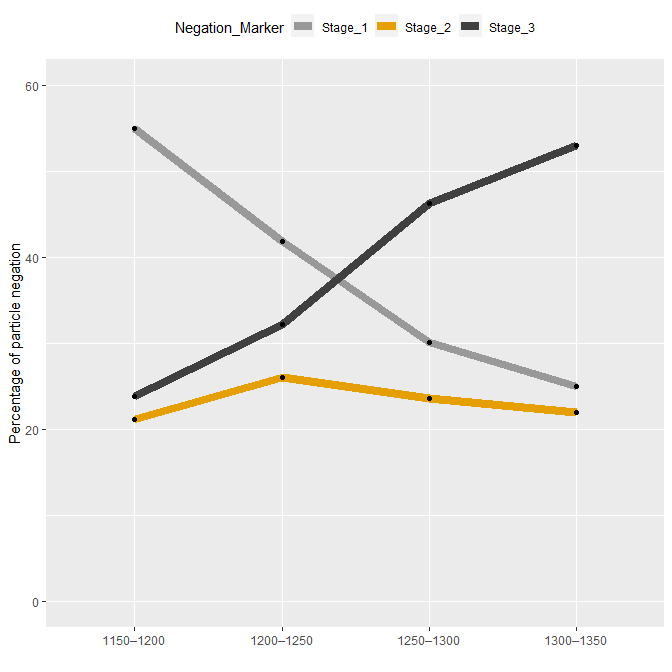
\includegraphics[width=7cm]{Diachron.png}
\end{figure}
    
\end{frame}

\subsection{Diatopic variation (ReM \& CAO)}
\begin{frame}
\frametitle{Our results}
\framesubtitle{Diatopic variation (ReM)}
    \begin{itemize}
        \item The omission of diatopic variation gives the impression that the classical \textit{Jespersen's Cycle} did not occur.
        \item Taking into account the \textbf{dialectal colouring} of the original texts, we get a \textbf{completely different picture} supporting \citet{schueler16,schueler17} and \citet{HertelimErscheinen}:
        \begin{itemize}
            \item MHG can be broken down into four major variants: Eastern \& Western Upper German and Eastern \& Western Central German.
            \item Bear in mind that the Eastern Central German dialects can only be meaningfully analysed in the last third of MHG (from 1250) due to the lack of traditional texts $\rightarrow$ we will largely \textbf{exclude ECG} from the discussion.
        \end{itemize}
        \item Now we can clearly see that the \textbf{negation change differs considerably} in the individual areas:
    \end{itemize}
\end{frame}


\begin{frame}
\frametitle{Our results}
\framesubtitle{Diatopic variation (ReM)}

\begin{small}
\begin{center}
\begin{tabular}{c c c | c c | c c}
\hline\hline
 & East UG. &  & West UG. & & West CG. & \\
 & Bipartite & Post & Bipartite & Post & Bipartite & Post\\
\hline
\alert{1150–1200} & \alert{785} & \alert{686} & \alert{47} & \alert{72} & 101 & 289 \\
1200–1250 & 154 & 459 & \alert{113} & \alert{115} & \alert{235} & \alert{47}\\
1250–1300 & 101 & 611 & 45 & 415 & \alert{413} & \alert{199}\\
1300–1350 & 59 & 869 & 56 & 310 & \alert{676} & \alert{527}\\
\hline
Total: & 1099 & 2625 & 261 & 912 & 1427 & 1064\\
 & total: & 3724 & total: & 1173 & total: & 2491\\
\hline\hline
\end{tabular}
\end{center}
\end{small}
\begin{center}
Table: Frequencies of stage II \& III negation in comparison
\end{center}

\end{frame}

\begin{frame}
\frametitle{Our results}
\framesubtitle{Diatopic variation (ReM)}

    \begin{itemize}
            \item \textbf{Upper German}: short peak between 1150 and 1200 in which the negation shifts from bipartite (\textit{ne ... niht}) to single, postverbal \textit{niht}. After 1250, almost every negated clause contains \textbf{\textit{niht} only} $\rightarrow$ transition to stage III
            \item \textbf{Western Central German}: \textbf{bipartite negation marker in its peak} from 1200 to the end of MHG. 
            \begin{itemize}
                \item The transition from stage II to III negation seems to take place after 1350. \textit{ne ... niht} stays the \textbf{main strategy} for expressing negation.
                \item The deviation between 1150 and 1200 is due to two single texts: \textit{Trier Versionen zum Interlinearpsalter} and \textit{Trier Psalmen} which behave more like WUG texts.
                \end{itemize}
    \end{itemize}
    
\centering    \textbf{ $\rightarrow$ Evidence for a stable stage II in MHG!}

\end{frame}

\subsection{In-depth analysis (ReM \& CAO)}
\begin{frame}
\frametitle{Our results}
\framesubtitle{Syntactic variation (ReM)}
    
    \begin{itemize}
        \item \textbf{V1 clauses are rare} – this is due to prosodic reasons, as we discussed earlier.
        \item \textbf{V2} is the \textbf{most frequent} verb order, but is \textbf{decreasing} until the end of MHG for the \textbf{favor of verb-later and verb-final clauses}.
        \item \textbf{VF seems to have a preservative effect}, as \citet[245]{behaghel18} already pointed out $\rightarrow$ we can observe a steady increase in VF-clauses (although V2 remains the most frequent position in total)
        \item matches the results of our CAO data and \citet{HertelimErscheinen}
        \item This pattern \textbf{doesn't seem to vary} between the four MHG dialects.
        
    \end{itemize}
    
\end{frame}

\begin{frame}
\frametitle{Our results}
\framesubtitle{Syntactic variation (ReM)}

\begin{center}
\begin{tabular}{c c c c}
\toprule
 & \textbf{Verb-initial} & \textbf{Verb-second} & \textbf{Verb-later/-final}\\
\hline
\hline
1150–1200 & 11 & \alert{124} & \alert{16}\\
1200–1250 & 3 & \alert{59} & \alert{21}\\
1250–1300 & 14 & \alert{44} & \alert{48}\\
1300–1350 & 14 & \alert{90} & \alert{57}\\ 
\hline
\hline
\textbf{Total:} & 42 & 317 & 142\\
\end{tabular}
\end{center}
\begin{center}
Table: Variation in verb order with the bipartite negation marker
\end{center}

\end{frame}

\begin{frame}{Our results}
\framesubtitle{Syntactic variation (CAO)}



\end{frame}

\begin{frame}{Our results}
\framesubtitle{Direction of clitic \textit{ne}}

\begin{itemize}
    \item In previous literature, it is sometimes mentioned that the preverbal marker (in combination with \textit{niht}) changes its direction when acting like a clitic (e.g. \citealt{Szczepaniak2010}).
    \item While being a proclitic element in the beginning (6), it can appear as an enclitic later on (7).
    \item This is most commonly explained with phonotactic reasons (sonority).
\end{itemize}

\pex[interpartskip=1ex]
\begingl
\gla Ein reine wif \textbf{enkan} nýt baz Verdýuen boeſer wive haz//
\glb a pure woman {\textsc{NEG}}=can \textsc{NEG} better earn evil women hatred//
\glft M357-G1 0a, 5409–5410 (Das Leben der Gräfin Yolanda von Vianden M)//
\endgl
\xe
\end{frame}

\begin{frame}{Our results}
\framesubtitle{Direction of clitic \textit{ne}}

\pex[interpartskip=1ex]
\begingl
\gla \textbf{ſine} uerſuchtenez an ſi niht mere//
\glb they={\textsc{NEG}} tried=it without her \textsc{NEG} more//
\glft M121V-G1 0a, 16768 (Kaiserchronik A, Manuscript V)//
\endgl
\xe

\end{frame}

\begin{frame}{Our results}
\framesubtitle{Direction of clitic \textit{ne}}

\begin{itemize}
    \item As you will see on the next slide, we couldn't observe such a change.
    \item However, something did change: \textbf{clitization} (at least on graphematic level) became much more scarce – after 1250, the separately written \textit{ne} is the most frequent variant (8).
\end{itemize}

\pex[interpartskip=1ex]
\begingl
\gla vvan ſie den gotiſ zorn . nivt \textbf{\textipa{\=i}} vorhtin//
\glb why they the God.{\textsc{GEN}} wrath {} \textsc{NEG} \textsc{NEG} feared//
\glft M065-G1 62aa, 6–7 (Linzer Entechrist)//
\xe

\end{frame}

\begin{frame}{Our results}
\framesubtitle{Direction of clitic \textit{ne}}

\begin{figure}[h]
\centering
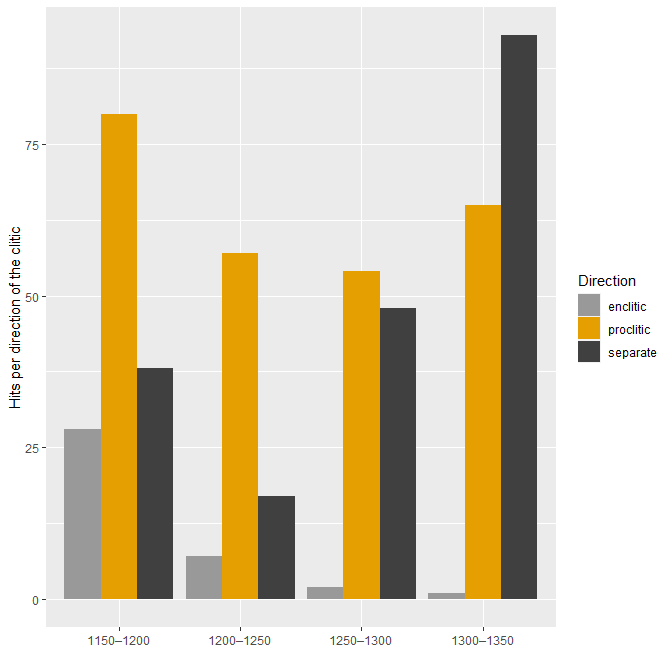
\includegraphics[width=7cm]{Clitic.png}
\end{figure}

\end{frame}

\begin{frame}{Our results}
\framesubtitle{Direction of clitic \textit{ne}}

\begin{figure}[h]
\centering
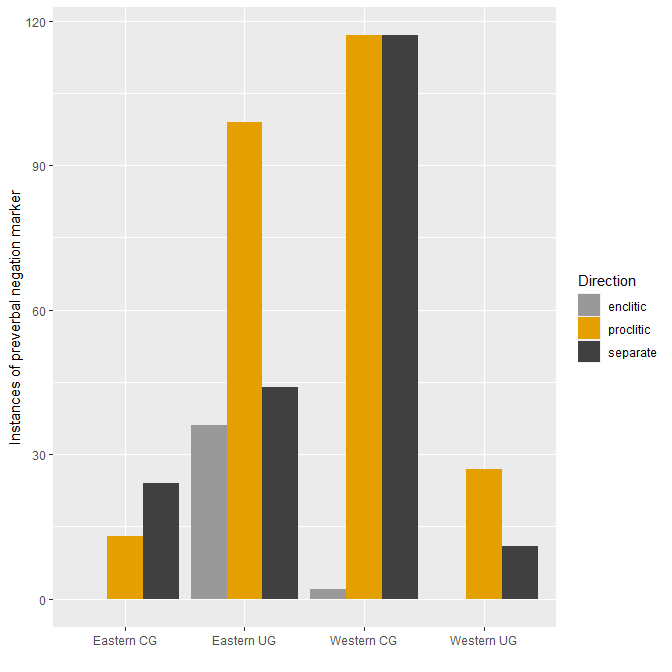
\includegraphics[width=7cm]{CliticD.png}
\end{figure}

\end{frame}

\begin{frame}{Our results}
\framesubtitle{Direction of clitic \textit{ne}}
\renewcommand{\arraystretch}{1.25}
\begin{center}\resizebox{\textwidth}{!}{%
\begin{tabular}{c c c c c c c}
\hline\hline
 & Eastern UG & & & Western CG & & \\
 & Proclitic & Separate & Enclitic & Proclitic & Separate & Enclitic\\
\hline
1150–1200 & 72 & 29 & 28 & 3 & 3 & 0\\
1200–1250 & 10 & 6 & 7 & 16 & 4 & 0\\
1250–1300 & 11 & 3 & 1 & 2 & 1 & 0\\
1300–1350 & 6 & 6 & 0 & 6 & 3 & 0\\
\hline
Insgesamt: & 99 & 44 & 36 & 27 & 11 & 0\\
\hline
 & Eastern CG & & & Western CG & &\\
 & Proclitic & Separate & Enclitic & Proclitic & Separate & Enclitic\\
\hline
1150–1200 & 0 & 0 & 0 & 5 & 6 & 0\\
1200–1250 & 0 & 0 & 0 & 31 & 7 & 0\\
1250–1300 & 7 & 9 & 0 & 34 & 35 & 1\\
1300–1350 & 6 & 15 & 0 & 47 & 69 & 1\\
\hline
Insgesamt: & 13 & 24 & 0 & 117 & 117 & 2\\
\hline\hline
\end{tabular}}
\end{center}

\begin{center}
Table: Diachrony of clitic \textit{ne} in MHG dialects
\end{center}

\end{frame}

\begin{frame}{Our results}
\framesubtitle{Direction of clitic \textit{ne}}

\begin{itemize}
    \item There was no such a thing as a change of directional change regarding clitization.
    \item Until 1250, proclitic \textit{ne} was the main variant; afterwards, separately written \textit{ne} became the most frequently used type.
    \item Concerning enclitic \textit{ne}: We only found a few instances of this type and they are almost always limited on early Bavarian texts.
\end{itemize}

\end{frame}

\begin{frame}
\frametitle{Summary \& conclusion}

\begin{itemize} 
\item \textbf{Illustration of diatopic, diachronic and syntactic variation} observed during \textbf{loss of the MHG bipartite negation marker} using mainly a large corpus (\textbf{ReM}), combined with the results of in-depth-study based on 13th century charters (\textbf{CAO})
\begin{itemize} 
\item \textbf{Upper German:} short use and early loss
\item \textbf{Western Central German:} long use and delayed loss
\item \textbf{Across all dialects:} early loss in V1 clauses due to prosodic reasons
\end{itemize} 
\end{itemize} 

\end{frame}

\begin{frame}
\frametitle{Summary \& conclusion}
\begin{itemize} 

\item \textbf{Comprehensive explanation} of this variation from a \textbf{phonological perspective}:
\begin{itemize} 
\item Analysis of the preverbal marker as a weak function word being reducted to Schwa
\item Schwa gets deleted during MHG (ENHG for WCG) $\rightarrow$ stray consonant /n/ or insertion of a \glqq Stützvokal\grqq{} $\rightarrow$ Reduction and deletion all over again
\item Final loss of remaining stray nasal due to prosodic reasons (sonority not matching; trochee as prosodic goal)
\end{itemize}
\item \textbf{Conclusion}: loss of \textit{ne/en} as well as syntactic variation can be explained with phonological/prosodical developments taking place during MHG! 
\end{itemize}
\end{frame}

\begin{frame}

\begin{center}

\begin{tikzpicture}[scale=3]
\duck[graduate=gray!20!black, laughing,speech={\textbf{Thanks for listening!}},bubblecolour=
white!60!blue,water=cyan!50!blue,
tassel=red!70!black,signpost=\scalebox{1.25}{
\parbox{2cm}{\textbf{\textcolor{black}{
\begin{center}{Grammar \& \\Corpora}\end{center}}}}},
signcolour=brown!70!gray,
signback=white!80!brow]
\end{tikzpicture}

\end{center}

\end{frame}

\begin{frame}[allowframebreaks]
\renewcommand\refname{}
\frametitle{References}

\printbibliography



\end{frame}

\begin{frame}{Appendix}
\framesubtitle{\textit{Jespersen's Cycle} in Eastern Central German (ECG)}

\begin{itemize}
    \item Due to the lack of traditional texts (not only within the ReM), ECG dialects can only be investigated from the second half of the 13\textsuperscript{th} century.
    \begin{itemize}
    \item ECG dialects are the result of the German colonization of the East (late 10\textsuperscript{th} – 13\textsuperscript{th} century)
    \item All in all, we can observe two periods of 50 years each: (i) 1250–1300 and (ii) 1300–1350.
    \item Therefore, the results should be treated with caution.
\end{itemize}
    \item What we can observe: During the \textbf{second half of the 13\textsuperscript{th} century}, the \textbf{bipartite negation marker is (still) in its peak}, but (most probably) already declining.
    \item However, this doesn't last for long: Within just 50 years, \textbf{the tide turns completely}: During the 14\textsuperscript{th} century, \textbf{\textit{niht}} rises quickly and \textbf{becomes the main negation strategy} (by far!) and displaces \textit{ne ... niht}.
    \end{itemize}

\end{frame}

\begin{frame}{Appendix}
\framesubtitle{\textit{Jespersen's Cycle} in Eastern Central German (ECG)}

\begin{center}
\begin{tabular}{c | c c}
\hline\hline
 & \multicolumn{2}{c}{Eastern Central German} \\
 & Bipartite & Postverbal\\
\hline
1150–1200 & \emptyset & \emptyset\\
1200–1250 & \emptyset & \emptyset\\
\alert{1250–1300} & \alert{113} & \alert{95}\\
\alert{1300–1350} & \alert{141} & \alert{537}\\
\hline
Total: & 254 & 632\\
\hline\hline
\end{tabular}
\end{center}
\begin{center}
Table: Frequencies of stage II and III in comparison (ECG only)
\end{center}

\end{frame}

\begin{frame}{Appendix}
\framesubtitle{\textit{Jespersen's Cycle} in Eastern Central German (ECG)}

\begin{itemize}
    \item As we have already discussed, the position of the finite verb does not (significantly) vary between the four major MHG dialect groups.
    \item Nevertheless, there is one conspicuous feature that is noticeable in Eastern Central German: We can observe \textbf{a (slightly) higher frequency of verb-initial clauses} in ECG.
    \begin{itemize}
        \item While VF clauses are rare (even during the last 50 years), V1 clauses are pretty common.
    \item However, this may be due to the \textbf{conjunct \textit{vnde}} which may occur in the form of \textit{en} or \textit{in}.
    \item In some cases, we can clearly decide whether \textit{ne} represents 'and' or 'not' – but in the majority of instances, we can't. 
        \end{itemize}
\end{itemize}
\end{frame}

\begin{frame}{Appendix}
\framesubtitle{\textit{Jespersen's Cycle} in Eastern Central German (ECG)}

\begin{footnotesize}
\begin{center}
\begin{tabular}{l c c c}
\toprule
 & \textbf{Verb-initial} & \textbf{Verb-second} & \textbf{Verbs-later/-final}\\
\hline
Eastern Upper German & 15 & 142 & 26\\
Western Upper German & 2 & 27 & 12\\
\alert{Eastern Central German} & \alert{12} & \alert{20} & \alert{6}\\
Western Central German & 13 & 128 & 98\\ 
\hline
\textbf{Total} & 42 & 317 & 142\\
\bottomrule
\end{tabular}
\end{center}
\end{footnotesize}

\begin{center}
Table: Verb position with the bipartite negation in the four major dialect gruops
\end{center}

\end{frame}

\begin{frame}
\frametitle{Appendix}
\framesubtitle{Using the ReM}
    
\begin{itemize}
    \item As we said earlier, the ReM is an annotated and PoS-tagged corpus consisting of approx. two million token.
    \item Although it exists since 2016, there are hardly any studies based on/using the ReM so far (\citealt{witzenhausen19, Schwarz2019, pickl21}).
    \item It makes use of ANNIS 3(\citealt{Krause2016}) and (in theory) allows for complex queries with e.g. syntactic boundaries, clause types and so on.
    \item Due to its features and its broad well-balanced texts, it can be used for diatopic and diachronic studies on MHG morphology and/or syntax.
    \item It is part of a larger series of reference corpora for Elder High (OHG, MHG, ENHG) and Low German (OS, MLG).
\end{itemize}
    
\end{frame}

\begin{frame}
\frametitle{Appendix}
\framesubtitle{Using the ReM}
    
\begin{itemize}
    \item With its sisters (\textit{Referenzkorpus Altdeutsch} (ReA); \textit{Referenzkorpus Mittelniederdeutsch/Niederrheinisch} (ReN; \citealt{ReNTeam2019}), it forms the joint network \textit{Deutsch Diachron Digital} (DDD)).
    \item However, from the perspective of a syntactician, there is \textbf{one major problem}:
    \item Unlike the others, the ReM \textbf{lacks syntactic annotations}: While we have the commands (e.g. parameter \textit{bound\_sent}), we can't use them because the underlying information is missing.
    \item For our study, we would have used sentence boundaries to exclude hits in which the bipartite negation marker is spread over two clauses.
\end{itemize}
    
\end{frame}

\begin{frame}
\frametitle{Appendix}
\framesubtitle{Using the ReM}
    
    \begin{itemize}
    \item Instead, we decided to work with distance parameters (e.g. no more than five token between the two negative elements) – definitely not the best option, but a sufficient and easy work-around.
    \item Although it works and has an acceptable precision, a lot of additional manual work is necessary.
    \end{itemize}
    
\end{frame}

\begin{frame}
\frametitle{Appendix}
\framesubtitle{Using the ReM}
    
    \begin{itemize}
    \item ANNIS query for the bipartite negation marker \textit{ne ... niht} (VF: \textit{niht ... ne}):
    \end{itemize}
    \vspace{-1cm}
\begin{center}
\begin{box}
lemma="ne" \&\\
lemma="niht" \&\\
pos="PTKNEG" \&\\
\#1 .1,6 \#2 \&\\
\#2 \_=\_ \#3\\ 
$|$\\
lemma= "ne" \&\\
lemma= "niht" \&\\
pos= "PTKNEG" \&\\
\#5 \.1,4 \#4 \&\\
\#5 \_=\_ \#6\\ 

\end{box}
\end{center}
    
\end{frame}
\end{document}